\documentclass[aspectratio=169]{beamer}

\mode<presentation>

\usepackage[utf8]{inputenc}
\usepackage[T1]{fontenc}	%makes å,ä,ö etc. proper symbols
\usepackage{amsmath}
\usepackage{graphicx}
\usepackage{xcolor}
\usepackage{listings}
\usepackage{multicol}
\usepackage{hyperref}

\definecolor{LundaGroen}{RGB}{00,68,71}
\definecolor{StabilaLila}{RGB}{85,19,78}
\definecolor{VarmOrange}{RGB}{237,104,63}

\definecolor{MagnoliaRosa}{RGB}{251,214,209}
\definecolor{LundaHimmel}{RGB}{204,225,225}
\definecolor{LundaLjus}{RGB}{255,242,191}

\usefonttheme{serif}
\usetheme{malmoe}
\setbeamercolor{palette primary}{bg=VarmOrange}
\setbeamercolor{palette quaternary}{bg=LundaGroen}
\setbeamercolor{background canvas}{bg=LundaLjus}
\setbeamercolor{structure}{fg=LundaGroen}

\usepackage[many]{tcolorbox}

\newtcolorbox{cross}{blank,breakable,parbox=false,
  overlay={\draw[red,line width=5pt] (interior.south west)--(interior.north east);
    \draw[red,line width=5pt] (interior.north west)--(interior.south east);}}

\lstset{language=[LaTeX]Tex,%C++,
    morekeywords={PassOptionsToPackage,selectlanguage},
    keywordstyle=\color{blue},%\bfseries,
    basicstyle=\small\ttfamily,
    %identifierstyle=\color{NavyBlue},
    commentstyle=\color{red}\ttfamily,
    stringstyle=\color{orange},
    numbers=left,%
    numberstyle=\scriptsize,%\tiny
    stepnumber=1,
    numbersep=8pt,
    showstringspaces=false,
    breaklines=true,
    %frameround=ftff,
    frame=single,
    belowcaptionskip=.75\baselineskip,
	tabsize=4
    %frame=L
}
\lstset{language=Python} 
\lstset{backgroundcolor=\color{white}}

\newcounter{uppgifter}

\begin{document}

\lstset{literate=
  {á}{{\'a}}1 {é}{{\'e}}1 {í}{{\'i}}1 {ó}{{\'o}}1 {ú}{{\'u}}1
  {Á}{{\'A}}1 {É}{{\'E}}1 {Í}{{\'I}}1 {Ó}{{\'O}}1 {Ú}{{\'U}}1
  {à}{{\`a}}1 {è}{{\`e}}1 {ì}{{\`i}}1 {ò}{{\`o}}1 {ù}{{\`u}}1
  {À}{{\`A}}1 {È}{{\'E}}1 {Ì}{{\`I}}1 {Ò}{{\`O}}1 {Ù}{{\`U}}1
  {ä}{{\"a}}1 {ë}{{\"e}}1 {ï}{{\"i}}1 {ö}{{\"o}}1 {ü}{{\"u}}1
  {Ä}{{\"A}}1 {Ë}{{\"E}}1 {Ï}{{\"I}}1 {Ö}{{\"O}}1 {Ü}{{\"U}}1
  {â}{{\^a}}1 {ê}{{\^e}}1 {î}{{\^i}}1 {ô}{{\^o}}1 {û}{{\^u}}1
  {Â}{{\^A}}1 {Ê}{{\^E}}1 {Î}{{\^I}}1 {Ô}{{\^O}}1 {Û}{{\^U}}1
  {œ}{{\oe}}1 {Œ}{{\OE}}1 {æ}{{\ae}}1 {Æ}{{\AE}}1 {ß}{{\ss}}1
  {ű}{{\H{u}}}1 {Ű}{{\H{U}}}1 {ő}{{\H{o}}}1 {Ő}{{\H{O}}}1
  {ç}{{\c c}}1 {Ç}{{\c C}}1 {ø}{{\o}}1 {å}{{\r a}}1 {Å}{{\r A}}1
  {€}{{\euro}}1 {£}{{\pounds}}1 {«}{{\guillemotleft}}1
  {»}{{\guillemotright}}1 {ñ}{{\~n}}1 {Ñ}{{\~N}}1 {¿}{{?`}}1
}

\lstset{escapeinside={(*@}{@*)}}

% NEW COMMANDS
\AtBeginSection[ ]
{
\begin{frame}{Outline}
	\begin{multicols}{2}
		\tableofcontents[currentsection]
	\end{multicols}
\end{frame}
}

\title{JSON}
\date{2024/25}
\author{Programmering 2}

\maketitle

\section{Dictionaries}

\subsection{Skapa en dictionary}

\begin{frame}[fragile]
\frametitle{Dictionaries}

En \lstinline{dictionary} i Python är en variant av \texttt{lista}. I en \texttt{lista} så kommer man åt varje element med dess index (position i listan) medan i en \lstinline{dictionary} kommer åt varje element med ett nyckelord.

\begin{lstlisting}
ordbok = {'CaK': 'Ketola', 'JoK': 'Kleimann'}
print(ordbok['CaK'])
>>> 'Ketola'
\end{lstlisting}

\end{frame}

\begin{frame}[fragile]
\frametitle{Dictionaries}
\framesubtitle{Keywords}

En så kallad \lstinline{key} behöver inte vara en sträng utan kan också vara ett tal:

\begin{lstlisting}
cities = {'Lund':125951, 3: 347949}
print(cities['Lund'])
>>> 125951
print(cities[3])
>>> 347949
\end{lstlisting}

\end{frame}

\subsection{Lägga till element}

\begin{frame}[fragile]
\frametitle{Dictionaries}
\framesubtitle{Lägga till värden}

Om man vill lägga till ett nytt värde i en \lstinline{dictionary} använder skriver man så här:

\begin{lstlisting}
cities = {}
cities['Lund'] = 125951
cities['Malmö'] = 347949
\end{lstlisting}

Så man anger nyckeln och vad som ska finnas på den nyckelns plats.

\end{frame}

\subsection{Plocka bort element}

\begin{frame}[fragile]
\frametitle{Dictionaries}
\framesubtitle{Plocka bort värden}

Det finns två sätt att plocka bort saker ur \lstinline{dictionaries}:

\begin{lstlisting}
cities = {'Lund': 125951, 'Malmö': 347949, 'Höör':16830}
cities.pop('Malmö') # plockar bort malmö
>>> 347949
cities.popitem() # Tar bort det senast tillagda elementet
>>> ('Höör', 16830)
\end{lstlisting}

\end{frame}

\subsection{Loopa genom dictionaries}

\begin{frame}[fragile]
\frametitle{Dictionaries}
\framesubtitle{Loopa genom en dictionary}

\begin{itemize}
	\item Du kan loopa genom en \lstinline{dictionary} tre sätt:
\end{itemize}

\begin{lstlisting}
ordlista = {'a':5, 'b':1, 'c':3, 'd':9}
# Med nycklar
for key in ordlista:
  print(ordlista[key])
\end{lstlisting}

\begin{lstlisting}
>>> 5
>>> 1
>>> 3
>>> 9
\end{lstlisting}

\end{frame}

\begin{frame}[fragile]
	\frametitle{Dictionaries}
	\framesubtitle{Loopa genom en dictionary}
	
	\begin{lstlisting}
ordlista = {'a':5, 'b':1, 'c':3, 'd':9}
# Med värden
for val in ordlista.values():
  print(val)
	\end{lstlisting}
	
	\begin{lstlisting}
>>> 5
>>> 1
>>> 3
>>> 9
\end{lstlisting}


\end{frame}

\begin{frame}[fragile]
	\frametitle{Dictionaries}
	\framesubtitle{Loopa igenom en dictionary}
	
	\begin{itemize}
		\item Man kan också använda \lstinline{enumerate} (detta fungerar också på vanliga listor):
	\end{itemize}
	
	\begin{lstlisting}
# Med enumerate
ordlista = {'a':5, 'b':1, 'c':3, 'd':9}

for val, key in enumerate(ordlista):
	print(val, key)
	\end{lstlisting}
	
	\begin{lstlisting}
>>> 5 a
>>> 1 b
>>> 3 c
>>> 9 d
\end{lstlisting}
	
	\begin{itemize}
		\item Med \lstinline{enumerate} får man ut både värdet och nyckeln.
	\end{itemize}
	
\end{frame}

\subsection{Övning}

\begin{frame}[fragile]
	\frametitle{Dictionaries}
	\framesubtitle{Övning}
	
	\begin{enumerate}
		\item Skapa dictionary:n nedanför
		\item Uppdatera elementet på plats \lstinline{"Malmö"} med ett
		\item Lägg till \lstinline{"Lund"} och ge det värdet 0.
	\end{enumerate}
	
	\begin{lstlisting}
eurovision = {"Stockholm": 2, "Göteborg": 1, "Malmö": 2}
	\end{lstlisting}
	
\end{frame}


\section{JSON}

\subsection{JavaScript objekt}

\begin{frame}[fragile]
\frametitle{JSON}
\framesubtitle{JavaScript Object Notation}

JSON är en standard för hur man modulerar data som skickas mellan datorer och ser ungefär ut som \lstinline{dictionaries} i Python.

\begin{lstlisting}
{
  "firstName": "Calle",
  "lastName": "Ketola",
  "work": {
    "workspace": "Hedda Anderssongymnasiet",
    "city": "Lund" 
  }
}
\end{lstlisting}

\end{frame}

\subsection{JSON och dictionaries}

\begin{frame}[fragile]
\frametitle{JSON}
\framesubtitle{Som en dict}

Om vi hade sparat \texttt{JSON} objektet som variabeln \texttt{calle} hade vi kunnat komma åt den som en vanlig \texttt{dictionary}

\begin{lstlisting}
print(calle.keys())
>>> dict_keys(["firstName", "lastName", "work"])
\end{lstlisting}

\begin{lstlisting}
for val in calle.values():
  print(val, end=", ")
>>> Calle, Ketola, {'workspace': 'Hedda Anderssongymnasiet', 'city': 'Lund'},
\end{lstlisting}

\end{frame}

\subsection{Dict i en dict}

\begin{frame}[fragile]
\frametitle{JSON}
\framesubtitle{Dictionary i en dictionary}

För att komma åt det som ligger i nyckeln \lstinline{"work"} så använder vi samma metod som med flerdimensionella listor:

\begin{lstlisting}
print(calle['work']['city'])
>>> Lund
\end{lstlisting}

\end{frame}

\subsection{Biblioteket json}

\begin{frame}[fragile]
\frametitle{JSON}
\framesubtitle{Biblioteket json}

För att kunna hantera JSON-objekt så behöver kan man importera biblioteket \texttt{json} som följer med i standardversionen av Python.

\begin{lstlisting}
import json
\end{lstlisting}

(De flesta bibliotek som jobbar med api:er har egna JSON moduler inbyggda så i praktiken behöver man sällan importera json)

\end{frame}

\begin{frame}[fragile]
\frametitle{JSON}
\framesubtitle{Biblioteket json}

Säg att vi har filen \texttt{data.json} som innehåller följande text:

\begin{lstlisting}
{
	"firstName":"Calle",
	"lastName": "Ketola",
	"work": {
		"workspace":"Hedda Anderssongymnasiet",
		"city": "Lund"
	}
}
\end{lstlisting}

\end{frame}

\begin{frame}[fragile]
\frametitle{JSON}
\framesubtitle{Biblioteket json}

För att läsa in den i Python gör vi så här:

\begin{lstlisting}
import json

with open("data.json") as f:
  data = json.load(f)

print(type(data))
>>> <class 'dict'>
print(data.keys())
>>> dict_keys(['firstName', 'lastName', 'work'])
\end{lstlisting}

\end{frame}

\section{Övningar}

\subsection{Blad 1}

\begin{frame}
	\frametitle{Övningar}
	\framesubtitle{Blad 1}
	
	\begin{enumerate}
		\item Skriv ut alla nycklar i variabeln eurovision
		\item Skriv ut alla nycklar med sina respektive värden i variabeln eurovision
		\item Variabeln antal är en dictionary med alfabetet. Använd den för att räkna hur många gånger varje bokstav förekommer i texten som är sparad i variabeln text.
		\item Vilken bokstav var vanligast i texten?
		\setcounter{uppgifter}{\value{enumi}}
	\end{enumerate}
	
	
\end{frame}

\subsection{Blad 2}

\begin{frame}
\frametitle{Övningar}
\framesubtitle{Blad 2}

\begin{enumerate}
	\setcounter{enumi}{\value{uppgifter}}
	\item Ladda ner filerna \texttt{data1.json}, \texttt{data2.json} och \texttt{data3.json} från Classroom.
	\item Läs in datan i filen \texttt{data1.json} i Python och skriv ut alla nycklar och all data.
	\item Läs in datan i filen \texttt{data2.json}.
	\item Hur många objekt finns det i data2-filen?
	\item Hur många av personerna jobbar i Lund?
	\setcounter{uppgifter}{\value{enumi}}
\end{enumerate}

\end{frame}

\subsection{Blad 3}

\begin{frame}
\frametitle{Övningar}
\framesubtitle{Blad 3}

\begin{enumerate}
	\setcounter{enumi}{\value{uppgifter}}
	\item Läs in datan i filen \texttt{data3.json}.
	\item Hur många videoklipp har användaren lagt upp?
	\item Vad är titeln på det längsta videoklippet?
	\item Skriv ut titeln på alla klipp som har fler \texttt{likes}+\texttt{dislikes} än \texttt{views}.
	\item All tid i videoklippen är angivna i sekunder. Skriv ut hur långt varje klipp är på formatet \texttt{hh:mm:ss - Titel}
	\setcounter{uppgifter}{\value{enumi}}
\end{enumerate}

\end{frame}

\subsection{Blad 4}

\begin{frame}
	\frametitle{Övningar}
	\framesubtitle{Blad 4}
	
	\begin{enumerate}
		\setcounter{enumi}{\value{uppgifter}}
		\item Presentera datan från \texttt{data2.json} med Tkinter.
		\item Presentera datan från \texttt{data3.json} med Tkinter.
	\end{enumerate}
	
	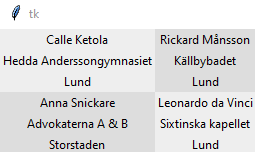
\includegraphics[width=.3\linewidth]{svar-data2.png}
	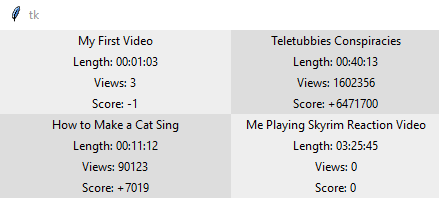
\includegraphics[width=.5\linewidth]{svar-data3.png}

\end{frame}



\end{document}